\scanpage{54}
% archive foliation: 53
\[
U\underset{\omega'}{\underbrace{\subset}}W\underset{\omega}{\underbrace{\subset}}V
\qquad\Omega(V/W)\wedge\Omega(V)\longrightarrow\Omega(W)
\]
\[
\mathrm{St}_{\omega}:\Omega(V)\unsure{\longrightarrow|\text{---}}\Omega(W)
\]
\[
\mathrm{St}_{\omega'}:\Omega(W)\text{---}\Omega(U)
\]
\[
\mathrm{St}_{\omega'}\mathrm{St}_{\omega}:\Omega(V)\longrightarrow\Omega(U)
\]
\[
I(\omega,\omega')\in\Omega
\]
\margin{$(\omega,\omega')\longmapsto\omega\times\omega'$}
\[
\Omega(V)\wedge\Omega(V')\longrightarrow\Omega(V\unsure{\wedge|\times}V')
\]
\[
\omega'\times\omega=(-1)^{\dim V.\dim V'}\deleted{\unsure{\Omega}}\omega\times\omega'
\]
\[
\deleted{\mathrm{St}(\omega)=\mathrm{St}(\omega')}
\]
\diagram{\begin{tikzcd}[column sep=small,row sep=small]
\mathbb{R}\arrow[d,phantom,"\cup"]\arrow[r,phantom,"\subset"] &
\mathbb{R}^2\arrow[d,phantom,"\cup"]\arrow[r,phantom,"\subset"] &
\mathbb{R}^3\arrow[d,phantom,"\cup"]\arrow[r,dash] &
\mathbb{R}^{n-1}\arrow[d,phantom,"\cup"]\arrow[r,phantom,"\subset"] &
\mathbb{R}^n\arrow[d,phantom,"\cup"]\\
\mathbb{R}^+\arrow[r,phantom,"\subset"] &
\mathbb{R}\times\mathbb{R}^+\arrow[r,phantom,"\subset"] &
\mathbb{R}^2\times\mathbb{R}^+\arrow[r,phantom,"\subset"] &
\mathbb{R}^{\unsure{n-2}}\times\mathbb{R}^+\arrow[r,phantom,"\subset"] &
\mathbb{R}^{n-1}\times\mathbb{R}^+
\end{tikzcd}}
\[
\unsure{\ell_1\wedge\text{---}\ell_{n-1}\wedge\ell_n|e_1\wedge\text{---}e_{n-1}\wedge e_n}
\qquad e_1\wedge\text{---}\wedge e_{n-1}\wedge e_n
\]
\[
\omega\times\omega'\qquad I(\omega,\omega')\qquad I(\omega',\omega)
\]
\[
\left\{\begin{array}{l}
\mathrm{St}(\omega\times\omega')=\inserted{\unsure{(-1)^q|(-1)^{?}}}\mathrm{St}(\omega)\times\omega'\\
\mathrm{St}(\omega\times\omega')=\deleted{\unsure{(-1)^p}}\omega\times\mathrm{St}\omega'
\end{array}\right.
\]
\[
\underbrace{e_1\text{---}e_p}\quad f_1\text{---}f_q
\]
\[
\mathrm{St}(e_1\text{---}e_{p-1}e_p f_1\text{---}f_q)
=(-1)^{\unsure{q}}e_1\text{---}e_{p-1}\widehat e_p f_1\unsure{\text{---}f_q}
\]
\[
e_1\ e_2\text{---}e_n
\]
\figure{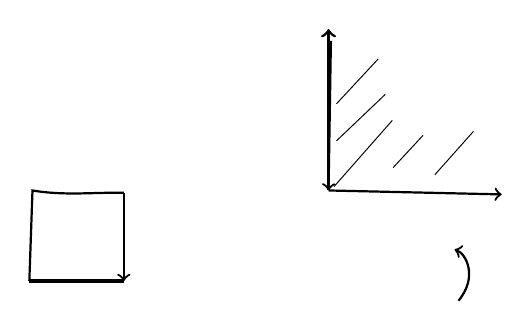
\begin{tikzpicture}[x=1cm,y=1cm]
\draw[line width=.8pt] (0,0)--(.04,1.15) .. controls (.45,1.08) and (.83,1.13) .. (1.2,1.12);
\draw[line width=.8pt,->] (1.2,1.12)--(1.2,0);
\draw[line width=1.2pt] (1.2,0)--(0,0);
\draw[line width=1pt,->] (3.8,1.15)--(3.8,3.2);
\draw[line width=.8pt,->] (3.83,3.05)--(3.8,1.15);
\draw[line width=.8pt,->] (3.8,1.15)--(6,1.1);
\draw[line width=.35pt] (3.9,2.25)--(4.43,2.82);
\draw[line width=.35pt] (3.9,1.78)--(4.52,2.37);
\draw[line width=.35pt] (3.87,1.2)--(4.61,2.04);
\draw[line width=.35pt] (4.62,1.44)--(5,1.85);
\draw[line width=.35pt] (5.15,1.35)--(5.64,1.9);
\draw[line width=.8pt,->] (5.45,-.25) .. controls (5.7,.05) and (5.55,.35) .. (5.4,.4);
\end{tikzpicture}}
